\chapter{Tutorial 1: Phenomenological Modeling}  

\section{Pendulum with implicit Euler time integration}

Start the SOFA scene file \emph{Spring\_EulerImplicit.scn} that describes a simple mass-spring system which is discretized using an implicit Euler scheme.

If you are using the pre-built Docker container this can be achieved by executing
\begin{lstlisting}[language=sh, breaklines=true]
$ cd /opt/sofa/bin 
\end{lstlisting}

\begin{lstlisting}[language=sh, breaklines=true]
$ ./runSofa /home/msml/tutorials/Tutorial1/Spring_EulerImplicit.scn
\end{lstlisting}

In order to see the spring-mass model as shown Fig. \ref{PendulumScreenshot}, please click \emph{All} in the tab \emph{View}. To animate a scene click on \emph{animate}. For moving a particle press \emph{shift} and click on the specified particle.

\begin{figure}[h]
  	\centering
    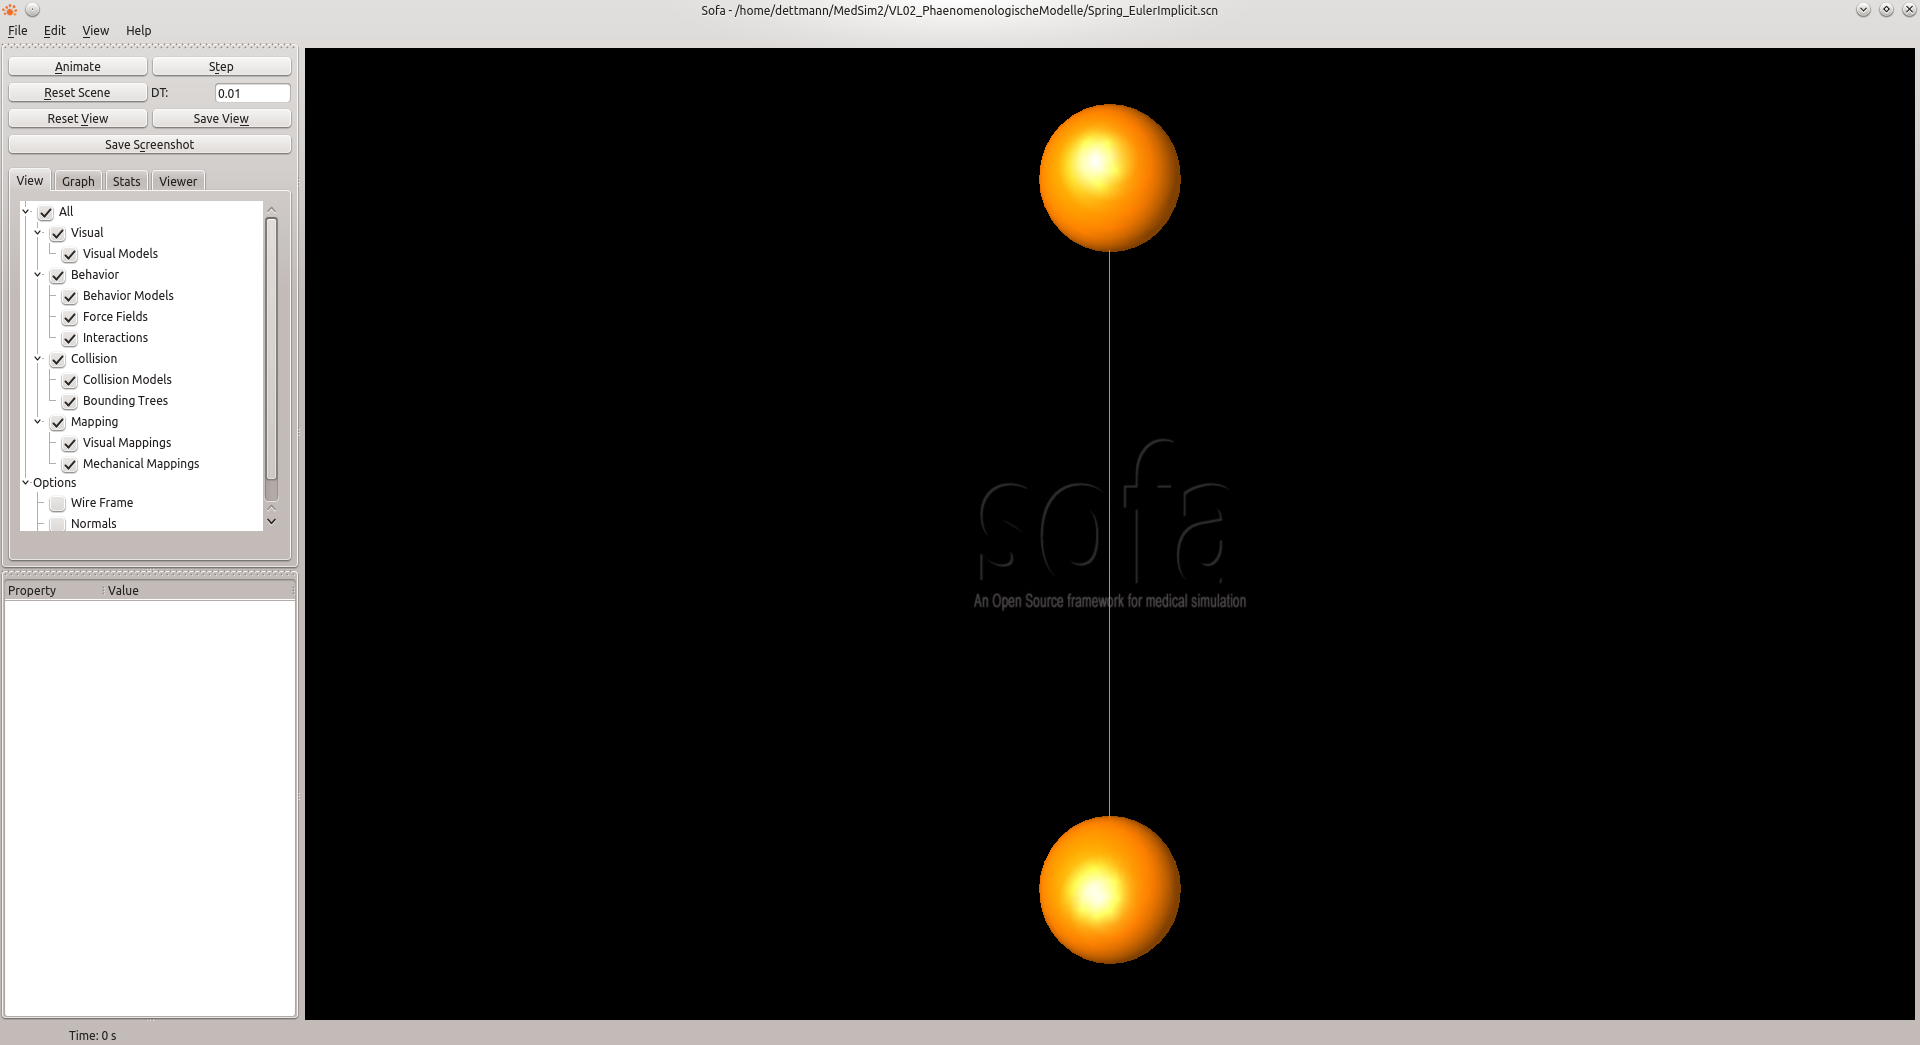
\includegraphics[width=\textwidth]{pictures/sofa_screenshot.png}
    \caption{SOFA framework running a simple pendulum simulation.}
    \label{PendulumScreenshot}
\end{figure}

Parametric studies can be used to get a better understanding of numerical methods. In order to analyze the implicit Euler technique, change the following input parameters
\begin{itemize}
	\item time step size dt in s [0.001, 0.01, 0.1, 1]
	\item stiffness $K_s$ and damping coefficient $K_d$ of the spring (spring='Id1, Id2, $K_s$, $K_d$, L')
\end{itemize}

The parameters can be changed by opening the SOFA scene file (.scn) in a suitable text editor, e.g.
\begin{lstlisting}[language=sh, breaklines=true]
$ geany /home/msml/tutorials/Tutorial1/Spring_EulerImplicit.scn &
\end{lstlisting}

While changing the parameters observe the behavior of the simulation. In particular, try to answer the following questions
\begin{itemize}
	\item How does the parameter effect the stability of the simulation?
	\item Does the frequency or amplitude change?
	\item How does the energy of the system behave over time?
\end{itemize}

\section{Pendulum with explicit Euler time integration}

The pendulum can also be discretized with an explicit Euler time integration scheme (\emph{Spring\_EulerImplicit.scn}). Repeat your analysis on this set-up. In particular, compare the behavior of the explicit and the implicit scheme. 
